\documentclass[border=6pt]{standalone}
\usepackage{fontspec,xeCJK,amsmath,amssymb,tikz,graphicx}
\usetikzlibrary{arrows.meta}\setmainfont{Arial}\setCJKmainfont{PingFang SC}
\definecolor{ink}{HTML}{203340}\definecolor{blue}{HTML}{147E91}\definecolor{pale}{HTML}{EFF6F5}\definecolor{line}{HTML}{D3E0DF}
\begin{document}\begin{tikzpicture}[x=1cm,y=1cm,every node/.style={text=ink,font=\fontsize{10}{13}\selectfont}]
\path[use as bounding box](0,0)rectangle(11,29.2);\fill[pale](0,0)rectangle(11,29.2);
\node[font=\fontsize{19}{23}\selectfont\bfseries]at(5.5,28.4){NeRF：把照片拟合成空间函数};
\node[text=blue]at(5.5,27.7){区域代码对应正文；虚线仅标阅读顺序};
\draw[rounded corners=6pt,draw=line,fill=white](.35,22.2)rectangle(10.65,27.0);\node[anchor=west,font=\fontsize{13}{16}\selectfont\bfseries]at(.65,26.45){A　照片与相机};
\node at(2.1,24.3){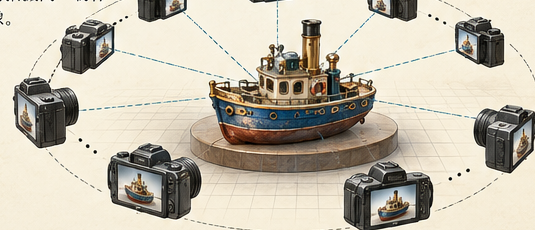
\includegraphics[width=2.75cm,height=2.7cm,keepaspectratio]{visual-1.png}};
\node[anchor=west]at(3.6,25.5){RGB + 相机内外参 $\to$ 像素射线};
\node[anchor=west]at(3.6,24.78){位置 $x\in\mathbb R^3$；单位方向 $d\in\mathbb R^3$};
\node[anchor=west]at(3.6,24.06){每条射线分层抽样；对应正文 §1--2};
\node[anchor=west]at(3.6,23.34){训练：拍过的相机；运行：新相机};
\draw[-{Stealth},dotted,draw=blue](5.5,22.2)--(5.5,21.8);
\draw[rounded corners=6pt,draw=line,fill=white](.35,17.0)rectangle(10.65,21.8);\node[anchor=west,font=\fontsize{13}{16}\selectfont\bfseries]at(.65,21.25){B　神经场查询};
\node at(2.1,19.1){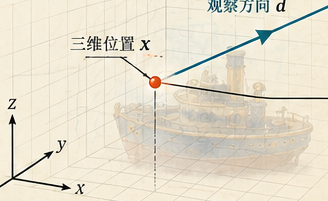
\includegraphics[width=2.75cm,height=2.7cm,keepaspectratio]{visual-2.png}};
\node[anchor=west]at(3.6,20.3){位置编码60维 $\to$ 8层256维MLP};
\node[anchor=west]at(3.6,19.580000000000002){位置 $\to$ 非负密度 $\sigma$ + 256维特征};
\node[anchor=west]at(3.6,18.86){特征 + 方向编码24维 $\to$ 128 $\to$ RGB};
\node[anchor=west]at(3.6,18.14){密度不依赖方向；对应正文 §3、§5.1};
\draw[-{Stealth},dotted,draw=blue](5.5,17.0)--(5.5,16.6);
\draw[rounded corners=6pt,draw=line,fill=white](.35,11.8)rectangle(10.65,16.6);\node[anchor=west,font=\fontsize{13}{16}\selectfont\bfseries]at(.65,16.05){C　沿射线合成};
\node at(2.1,13.900000000000002){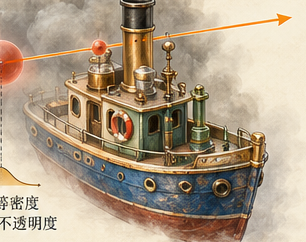
\includegraphics[width=2.75cm,height=2.7cm,keepaspectratio]{visual-3.png}};
\node[anchor=west]at(3.6,15.100000000000001){$\alpha_i=1-\exp(-\sigma_i\delta_i)$};
\node[anchor=west]at(3.6,14.38){前方透射 $T_i=\prod_{j<i}(1-\alpha_j)$};
\node[anchor=west]at(3.6,13.660000000000002){像素 $C=\sum_i T_i\alpha_i c_i$};
\node[anchor=west]at(3.6,12.940000000000001){同一计算供训练和新视角；正文 §4};
\draw[-{Stealth},dotted,draw=blue](5.5,11.8)--(5.5,11.4);
\draw[rounded corners=6pt,draw=line,fill=white](.35,6.599999999999999)rectangle(10.65,11.399999999999999);\node[anchor=west,font=\fontsize{13}{16}\selectfont\bfseries]at(.65,10.849999999999998){D　粗细采样与训练};
\node at(2.1,8.7){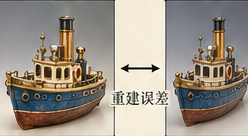
\includegraphics[width=2.75cm,height=2.7cm,keepaspectratio]{visual-4.png}};
\node[anchor=west]at(3.6,9.899999999999999){粗网64点 $\to$ 权重 $w_i=T_i\alpha_i$};
\node[anchor=west]at(3.6,9.179999999999998){按权重另采128点；细网查192点};
\node[anchor=west]at(3.6,8.459999999999999){粗/细像素平方误差 $\to$ 两网参数};
\node[anchor=west]at(3.6,7.739999999999998){训练每批4096射线；对应正文 §5.2--5.3};
\draw[-{Stealth},dotted,draw=blue](5.5,6.599999999999999)--(5.5,6.199999999999998);
\draw[rounded corners=6pt,draw=line,fill=white](.35,1.3999999999999995)rectangle(10.65,6.199999999999999);\node[anchor=west,font=\fontsize{13}{16}\selectfont\bfseries]at(.65,5.6499999999999995){E　新视角与检验};
\node at(2.1,3.499999999999999){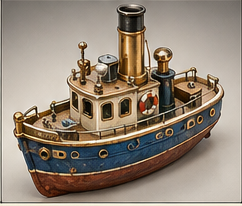
\includegraphics[width=2.75cm,height=2.7cm,keepaspectratio]{visual-5.png}};
\node[anchor=west]at(3.6,4.699999999999999){固定网络，换相机 $\to$ A/B/C/D的采样};
\node[anchor=west]at(3.6,3.9799999999999995){不再梯度更新；细网输出新视角RGB};
\node[anchor=west]at(3.6,3.2599999999999993){PSNR/SSIM/LPIPS；消融编码/方向/采样};
\node[anchor=west]at(3.6,2.539999999999999){静态场景外观；对应正文 §6--7};
\end{tikzpicture}\end{document}